\chapter{Prostor}

\section{Pseudometrický prostor, metrický prostor}

Mějme množinu prvků \(M\) a funkci \(d: M \times M \rightarrow \mathbb{R}\), která určuje vzdálenost dvou prvků z \(M\).

\begin{equation}
\label{eq:pseudometricky_prostor_definice_1}
\forall u \in M : d(u, u) = 0
\end{equation}

\begin{equation}
\label{eq:pseudometricky_prostor_definice_2}
\forall u, v \in M : d(u, v) = d(v, u)
\end{equation}

\begin{equation}
\label{eq:pseudometricky_prostor_definice_3}
\forall u, v, w \in M : d(u, v) \leq d(u, w) + d(w, v)
\end{equation}

Pokud funkce \(d\) splňuje podmínky \eqref{eq:pseudometricky_prostor_definice_1} - \eqref{eq:pseudometricky_prostor_definice_3}, pak se nazývá pseudometrika a dvojice \((M, d)\) pseudometrický prostor.

Podmínka \eqref{eq:pseudometricky_prostor_definice_1} říká, že vzdálenost totožných prvků je nulová. Podmínka \eqref{eq:pseudometricky_prostor_definice_2} znamená symetrii vzdálenosti a \eqref{eq:pseudometricky_prostor_definice_3} je trojúhelníková nerovnost.

Provedeme-li v rovnici \eqref{eq:pseudometricky_prostor_definice_3} subsstituci \(u = v = x, w = y\), a využijeme podmínky \eqref{eq:pseudometricky_prostor_definice_1} a \eqref{eq:pseudometricky_prostor_definice_2},
tak odvodíme nezápornost vzdálenosti.

\begin{equation}
\begin{split}
\forall x, y \in M : d(x, x) \leq d(x, y) + d(y, x) \\
\forall x, y \in M : 0 \leq 2 \cdot d(x, y) \\
\forall x, y \in M : d(x, y) \geq 0
\end{split}
\end{equation}

Pokud pseudometrický prostor splňuje navíc podmínku \eqref{eq:metricky_prostor_definice_1}, pak jej nazýváme metrickým prostorem.

\begin{equation}
\label{eq:metricky_prostor_definice_1}
\forall u, v \in M : d(u, v) = 0 \rightarrow u = v
\end{equation}

V~pseudometrickém prostoru tedy mohou existovat různé prvky s~nulovovou vzdáleností, v~metrickém prostoru je to vyloučeno.

\section{Euklidovský prostor, kartézský systém souřadnic}

Začněme definicí Euklidovského prostoru.

\begin{fact}
Definice: Euklidovský prostor \(E_n\) je metrický prostor, jehož prvky jsou body, v~němž můžeme zavést kartézský systém souřadnic a~v~němž platí metrika daná vztahem \eqref{eq:euklidovsky_prostor_metrika}.

\begin{equation}
\label{eq:euklidovsky_prostor_metrika}
d(A, B) = \sqrt{\sum_{i=1}^{n} (B_i - A_i)^2}
\end{equation}
\end{fact}

Euklidovský prostor je tedy prostor tvořený body. Můžeme zde zavést kartézský systém souřadnic, který každému bodu \(X\) přiřazuje \(n\)-tici reálných čísel \(X_i\). Říkáme, že se jedná o~\(n\)-rozměrný prostor.
Kartézský systém souřadnic není jediný možný, později si ukážeme, jak zavést jiné systémy souřadnic. Je pravděpodobné, že čtenář je s~kartézskou soustavou souřadnic podrobně seznámen. Předpokládejme ale nyní,
že o~ní nic nevíme a~ukážeme si, co vše lze z~rovnice \eqref{eq:euklidovsky_prostor_metrika} odvodit.

Především si všimněme, že ve vztahu \eqref{eq:euklidovsky_prostor_metrika} vystupují pouze rozdíly souřadnic. To znamená, že máme-li soustavu bodů,
pak přičtením konstantní \(n\)-tice ke všem jejich souřadnicím se vzájemné vzdálenosti bodů nezmění. Můžeme tedy soustavu bodů libovolně posunout a~jejich vzájemná poloha zůstane nezměněna. Toto je vlastnost Euklidovského
prostoru jako takového, ne jen soustavy souřadnic. To se může zdát samozřejmé, ale například teorie relativity předpokládá, že prostor může být deformovaný a~tuto vlastnost nemá. Tím jsme odvodili první fakt:

\begin{fact}
Euklidovský prostor \(E_n\) je invariantní vůči posunutí.
\end{fact}

Zavedeme označení
\eqref{eq:vektor_rozdil_bodu} a~veličinu \(\vectpoints{AB}\) nazveme vektorem. Vektor se v~některé literatuře označuje tučně, v~některé šipkou nad vektorem. V~této knize budeme vektory označovat tučně s~výjimkou vektoru
utvořeného jako rozdíl dvou bodů - ten označíme šipkou nad oněmi dvěma body. Pokud je daný vektor jednotkový (jeho velikost je rovna 1), pak nad ním
nakreslíme stříšku.

Velikost vektoru definujeme pomocí vztahu \eqref{eq:vektor_velikost}. Tím se nám definice \eqref{eq:euklidovsky_prostor_metrika} zjednoduší na \eqref{eq:euklidovsky_prostor_metrika_vektor}.

\begin{equation}
\label{eq:vektor_rozdil_bodu}
\vectpoints{AB} = (B_1 - A_1, B_2 - A_2, ..., B_n - A_n)
\end{equation}

\begin{equation}
\label{eq:vektor_velikost}
|\vect{u}| = \sqrt{\sum_{i=1}^{n} u_i^2}
\end{equation}

\begin{equation}
\label{eq:euklidovsky_prostor_metrika_vektor}
d(A, B) = |\vectpoints{AB}|
\end{equation}

Graficky budeme vektor reprezentovat pomocí šipky vedoucí od počátečního ke koncovému bodu, jak je vidět na obrázku~\ref{img:vektor_graficky}.

\begin{figure}[!h]
\centering
\begin{tikzpicture}
\draw[->] (0, 0) -- (2, 2);
\draw (0, 0) node[anchor=east]{A};
\draw (2, 2) node[anchor=west]{B};
\draw (1, 1) node[anchor=south east]{\(\vectpoints{AB}\)};
\end{tikzpicture}
\caption{Vektor}
\label{img:vektor_graficky}
\end{figure}

Mějme 3 body - A, B, C. Vidíme, že \(i\)-tá souřadnice vektoru \(\vectpoints{AB}\) je \(\vectpoints{AB}_i = B_i - A_i\), \(i\)-tá souřadnice vektoru \(\vectpoints{BC}\) je \(\vectpoints{BC}_i = C_i - B_i\) a~\(i\)-tá souřadnice vektoru \(\vectpoints{AC}\) je \(\vectpoints{AC}_i = C_i - A_i = (B_i - A_i) + (C_i - B_i) = \vectpoints{AB}_i + \vectpoints{BC}_i\). Můžeme proto zavést sčítání vektorů vztahem \eqref{eq:euklidovsky_prostor_vektor_soucet}.

\begin{figure}[!h]
\centering
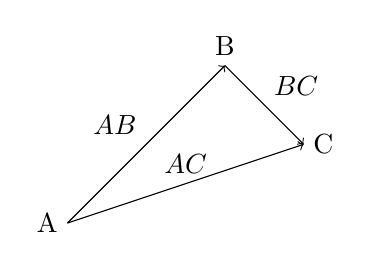
\begin{tikzpicture}
\draw[->] (0, 0) -- (2, 2);
\draw[->] (2, 2) -- (3, 1);
\draw[->] (0, 0) -- (3, 1);
\draw (0, 0) node[anchor=east]{A};
\draw (2, 2) node[anchor=south]{B};
\draw (3, 1) node[anchor=west]{C};
\draw (1, 1) node[anchor=south east]{\(\vectpoints{AB}\)};
\draw (2.5, 1.5) node[anchor=south west]{\(\vectpoints{BC}\)};
\draw (1.5, 0.5) node[anchor=south]{\(\vectpoints{AC}\)};
\end{tikzpicture}
\caption{Součet vektorů}
\label{img:soucet_vektoru}
\end{figure}

\begin{equation}
\label{eq:euklidovsky_prostor_vektor_soucet}
\vect{u} + \vect{v} = (u_1 + v_1, u_2 + v_2, ..., u_n + v_n)
\end{equation}

Dále definujme nulový vektor \(\vect{0}\) tak, že pokud jej přičteme k~libovolnému vektoru \(\vect{u}\), tak se nezmění. Tedy:

\begin{equation}
\begin{split}
\vect{u} + \vect{0} = \vect{u} \\
(u_1 + 0_1, u_2 + 0_2, ..., u_n + 0_n) = (u_1, u_2, ..., u_n ) \\
\vect{0} = (0, 0, ...)
\end{split}
\end{equation}

Vidíme, že nulový vektor má všechny složky nulové. Dosadíme-li jej do definice velikosti vektoru \eqref{eq:vektor_velikost}, tak vidíme, že \(|\vect{0}| = 0\). Navíc vidíme, že se jedná o~jediný vektor s~nulovou velikostí. Ve vztahu \eqref{eq:vektor_velikost} se totiž vyskytuje součet druhých mocnin složek vektoru. Aby tento součet mohl být nulový, tak každá složka musí být nulová. Také to tedy znamená, že nulovou metriku mohou mít jen stejné body Euklidovského prostoru. Dokázali jsme tak platnost podmínky \eqref{eq:metricky_prostor_definice_1}.

Opačný vektor \(-\vect{u}\) zavedeme jako vektor, který když přičteme k~vektoru \(\vect{u}\), tak získáme nulový vektor. Takto to bude odpovídat běžné algebře:

\begin{equation}
\begin{split}
\vect{u} + (-\vect{u}) = \vect{0} \\
(u_1 + (-\vect{u})_1, u_2 + (-\vect{u})_2, ..., u_n + (-\vect{u})_n) = (0, 0, ...) \\
-\vect{u} = (-u_1, -u_2, ..., -u_n)
\end{split}
\end{equation}

Rozdíl vektorů zavedeme jako přičtení opačného vektoru vztahem \eqref{eq:euklidovsky_prostor_vektor_rozdil}. Takto to bude odpovídat běžným pravidlům algebry.

\begin{equation}
\label{eq:euklidovsky_prostor_vektor_rozdil}
\vect{u} - \vect{v} = \vect{u} + (-\vect{v})= (u_1 - v_1, u_2 - v_2, ..., u_n - v_n)
\end{equation}

Přirozeně můžeme zavést násobení vektoru skalárem, aby odpovídalo sčítání příslušného počtu shodných vektorů. Získáme tak vztah \eqref{eq:euklidovsky_prostor_vektor_nasobeni}, který je kompatibilní se sčítáním a odečítáním vektorů:

\begin{equation}
\label{eq:euklidovsky_prostor_vektor_nasobeni}
\alpha \cdot \vect{u} = (\alpha \cdot u_1, \alpha \cdot u_2, ..., \alpha \cdot u_n)
\end{equation}


Protože jsme zavedli operace s~vektory tak, že provádíme běžné algebraické operace s~\(n\)-ticemi čísel po jednotlivých složkách, tak běžná pravidla algebry budou platit i~pro operace s~vektory. Neměla by nás proto překvapit následující pravidla. Čtenář si je může ověřit sám rozepsáním jednotlivých operací:

\begin{fact}
\begin{equation}
\label{eq:euklidovsky_prostor_definice_nuloveho_vektoru}
\vect{u} + \vect{0} = \vect{u}
\end{equation}

\begin{equation}
\label{eq:euklidovsky_prostor_definice_opacneho_vektoru}
\vect{u} + (-\vect{u}) = \vect{0}
\end{equation}

\begin{equation}
\label{eq:euklidovsky_prostor_definice_odecitani_vektoru}
\vect{u} - \vect{v} = \vect{u} + (-\vect{v})
\end{equation}

\begin{equation}
\label{eq:euklidovsky_prostor_vektor_asociativita_scitani}
\vect{u} + (\vect{v} + \vect{w}) = (\vect{u} + \vect{v}) + \vect{w}
\end{equation}

\begin{equation}
\label{eq:euklidovsky_prostor_definice_nasobeni}
\sum_{i=1}^n \vect{u} = n \cdot \vect{u}
\end{equation}

\begin{equation}
\label{eq:euklidovsky_prostor_vektor_opacny}
-\vect{u} = (-1) \cdot \vect{u}
\end{equation}

\begin{equation}
\label{eq:euklidovsky_prostor_vektor_distribuce_scitani}
\alpha \vect{u} + \beta \vect{u} = (\alpha + \beta) \cdot \vect{u}
\end{equation}

\begin{equation}
\label{eq:euklidovsky_prostor_vektor_distribuce_nasobeni}
\alpha \vect{u} + \alpha \vect{v} = \alpha \cdot (\vect{u} + \vect{v})
\end{equation}

\begin{equation}
\label{eq:euklidovsky_prostor_asociativita_nasobeni}
\alpha (\beta \vect{u}) = (\alpha \beta) \vect{u}
\end{equation}
\end{fact}

Každý nenulový vektor můžeme tzv. normalizovat - podělit jej jeho velikostí. Získáme tak jednotkový vektor \(\unitvect{u} = \frac{\vect{u}}{|\vect{u}|}\). Nebo jinak, každý nenulový vektor můžeme zapsat ve tvaru \(\vect{u} = |\vect{u}| \cdot \unitvect{u}\). Vektor \(\vect{u}\) jsme tak rozdělili na složku určující jeho velikost a~na složku určující jeho směr.

Ukazuje se, že ve výpočtech se často vyskytuje výraz  \(\sum_{i=1}^{n} u_i \cdot v_i\).
Nazveme jej skalárním součinem vektorů \(\vect{u}\) a \(\vect{v}\) a~označíme ho \(\vect{u} \cdot \vect{v}\).
Pokud jsou vektory nenulové, pak je můžeme normalizovat: \(\unitvect{u} = \frac{\vect{u}}{|\vect{u}|}\), \(\unitvect{v} = \frac{\vect{v}}{|\vect{v}|}\).

Prozkoumejme, jakých hodnot může nabývat skalární součin \(\unitvect{u} \cdot \unitvect{v}\). Ve vztahu \eqref{eq:skalarni_soucin_1} jsme skalární součin
vyjádřili pomocí sumy, kterou jsme dále upravovali. Využili jsme faktu, že \(\sum_{i=1}^{n} \hat{u}_i^2 = \sum_{i=1}^{n} \hat{v}_i^2 = 1\), protože vektory
\(\unitvect{u}\) a \(\unitvect{v}\) jsou jednotkové. Všimněme si, že \(\sum_{i=1}^{n} (\hat{u}_i + \hat{v}_i)^2\) je součet druhých mocnin členů
\(\hat{u}_i + \hat{v}_i\), proto je určitě nezáporný. Výraz \eqref{eq:skalarni_soucin_1} nabývá minimální hodnoty \(-1\) pouze pokud je suma nulová, tedy pokud každý je nulový, tedy pokud
\(\hat{u}_i = -\hat{v}_i\). Proto pro skalární součin (obecně nejednotkových) vektorů platí \(\vect{u} \cdot \vect{v} = |\vect{u}| \cdot \unitvect{u} \cdot |\vect{v}| \cdot \unitvect{v} \geq -|\vect{u}| \cdot |\vect{v}|\)
a~minimální hodnoty \(-|\vect{u}| \cdot |\vect{v}|\) nabývá právě tehdy pokud \(\unitvect{u} = -\unitvect{v}\), tedy pokud vektory \(\vect{u}\) a \(\vect{v}\) mají opačný směr.

\begin{equation}
\label{eq:skalarni_soucin_1}
\begin{split}
\unitvect{u} \cdot \unitvect{v} = \sum_{i=1}^{n} \hat{u}_i \cdot \hat{v}_i = \frac{1}{2} \sum_{i=1}^{n} 2 \cdot \hat{u}_i \cdot \hat{v}_i = \\
\frac{1}{2} \sum_{i=1}^{n} \left(\hat{u}_i^2 + 2 \cdot \hat{u}_i \cdot \hat{v}_i + \hat{v}_i^2 - \hat{u}_i^2 - \hat{v}_i^2 \right) = \\
\frac{1}{2} \sum_{i=1}^{n} (\hat{u}_i + \hat{v}_i)^2 - \frac{1}{2} \sum_{i=1}^{n} \hat{u}_i^2 - \frac{1}{2} \hat{v}_i^2 = \\
\frac{1}{2} \sum_{i=1}^{n} (\hat{u}_i + \hat{v}_i)^2 - \frac{1}{2} - \frac{1}{2} =  \\
\frac{1}{2} \sum_{i=1}^{n} (\hat{u}_i + \hat{v}_i)^2 - 1 \geq -1
\end{split}
\end{equation}

Skalární součin můžeme vyjádřit také pomocí vztahu \eqref{eq:skalarni_soucin_2}. Postupovali jsme obdobně jako v~minulém případě, ale tentokrát
vidíme, že skalární součin jednotkových vektorů nabývá maximální hodnoty \(1\) pouze pokud \(\hat{u}_i = \hat{v}_i\). Proto pro skalární součin (obecně nejednotkových) vektorů platí \(\vect{u} \cdot \vect{v} = |\vect{u}| \cdot \unitvect{u} \cdot |\vect{v}| \cdot \unitvect{v} \leq |\vect{u}| \cdot |\vect{v}|\)
a~maximální hodnoty \(|\vect{u}| \cdot |\vect{v}|\) nabývá právě tehdy pokud \(\unitvect{u} = \unitvect{v}\), tedy pokud vektory \(\vect{u}\) a \(\vect{v}\) mají stejný směr.

\begin{equation}
\label{eq:skalarni_soucin_2}
\begin{split}
\unitvect{u} \cdot \unitvect{v} = \sum_{i=1}^{n} \hat{u}_i \cdot \hat{v}_i = -\frac{1}{2} \sum_{i=1}^{n} -2 \cdot \hat{u}_i \cdot \hat{v}_i = \\
-\frac{1}{2} \sum_{i=1}^{n} \left(\hat{u}_i^2 - 2 \cdot \hat{u}_i \cdot \hat{v}_i + \hat{v}_i^2 - \hat{u}_i^2 - \hat{v}_i^2 \right) = \\
-\frac{1}{2} \sum_{i=1}^{n} (\hat{u}_i - \hat{v}_i)^2 + \frac{1}{2} \sum_{i=1}^{n} \hat{u}_i^2 + \frac{1}{2} \hat{v}_i^2 = \\
-\frac{1}{2} \sum_{i=1}^{n} (\hat{u}_i + \hat{v}_i)^2 + \frac{1}{2} + \frac{1}{2} =  \\
-\frac{1}{2} \sum_{i=1}^{n} (\hat{u}_i - \hat{v}_i)^2 + 1 \leq 1
\end{split}
\end{equation}

Souřadnice bodů a~vektorů jsou pro nás zatím jen \(n\)-tice čísel, nevíme, co si před nimi představit. Musíme nějakým způsobem definovat přímku a~úhly.

Zamysleme se nejdříve jak zavést obecnou definici úsečky tak, aby obstála i~v~zakřiveném prostoru. Představme si, že bychom zedníkovi vytyčili 2 body tak, že bychom do země zatloukly 2 kolíky, a~chtěli po něm, aby mezi nimi vytyčil
úsečku. Vzal by provaz, napnul by ho mezi kolíky a~řekl by nám, že provaz tvoří úsečku. Důležité je právě to, že by provaz napnul - tím by zajistil, že ze všech možných drah mezi oběma kolíky povede po dráze, která má
nejkratší vzdálenost. Takto můžeme zavést definici úsečky v~jakémkoli metrickém prostoru. Přesnou definici křivky si nechme na později.

\begin{fact}
Úsečka je křivka mezi dvěma body, která má ze všech možných křivek minimální délku.
\end{fact}

Abychom zjistili, kdy tento případ nastává, tak se podívejme na velikost součtu 2 vektorů.

\begin{equation}
\label{eq:delka_souctu_vektoru}
\begin{split}
|\vect{u} + \vect{v}|^2 = \sum_{i=1}^{n} (u_i + v_i)^2 = \sum_{i=1}^{n} u_i^2 + 2 \sum_{i=1}^{n} u_i \cdot v_i + \sum_{i=1}^{n} v_i^2 = \\
|\vect{u}|^2 + 2 \cdot \vect{u} \cdot \vect{v} + |\vect{v}|^2
\end{split}
\end{equation}

Dosadíme-li tyto meze skalárního součinu do vztahu \eqref{eq:delka_souctu_vektoru}, tak vidíme, že 

\begin{equation}
\begin{split}
|\vect{u}|^2 - 2 \cdot |\vect{u}| \cdot |\vect{v}| + |\vect{v}|^2 \leq |\vect{u} + \vect{v}|^2 \leq
|\vect{u}|^2 + 2 \cdot |\vect{u}| \cdot |\vect{v}| + |\vect{v}|^2 \\
(|\vect{u}| - |\vect{v}|)^2 \leq |\vect{u} + \vect{v}|^2 \leq
|(\vect{u}|+ |\vect{v}|)^2 \\
||\vect{u}| - |\vect{v}|| \leq |\vect{u} + \vect{v}| \leq
|\vect{u}|+ |\vect{v}|
\end{split}
\end{equation}

Uvedenému závěru se říká trojúhelníkové nerovnosti.
Vidíme také, že je splněna podmínka \eqref{eq:pseudometricky_prostor_definice_3}, kterou jsme kladli na metriku v~pseudometrickém prostoru. Splnění ostatních podmínek nebudeme rozebírat, čtenář si je může triviálně ověřit sám. Dále vidíme, že aby platilo \(|\vect{u} + \vect{v}| = |\vect{u}| + |\vect{v}|\), tak
je nutné, aby \(\unitvect{u} = \unitvect{v}\).

Mějme tedy 2 body \(A\) a~\(B\), které představují konce úsečky \(AB\). Bod \(X\) na ní leží pokud:

\begin{equation}
\begin{split}
\frac{\vectpoints{AX}}{|\vectpoints{AX}|} = \frac{\vectpoints{XB}}{|\vectpoints{XB}|} \\
\frac{\vectpoints{AX}}{|\vectpoints{AX}|} = \frac{\vectpoints{AB} - \vectpoints{AX}}{|\vectpoints{XB}|} \\
\vectpoints{AX} \cdot |\vectpoints{XB}| = \vectpoints{AB} \cdot |\vectpoints{AX}| - \vectpoints{AX} \cdot |\vectpoints{AX}| \\
\vectpoints{AX} \cdot |\vectpoints{XB}| + \vectpoints{AX} \cdot |\vectpoints{AX}| = \vectpoints{AB} \cdot |\vectpoints{AX}| \\
\vectpoints{AX} = \vectpoints{AB} \cdot \frac{|\vectpoints{AX}|}{|\vectpoints{XB}| + |\vectpoints{AX}|} \\
\vectpoints{AX} = \vectpoints{AB} \cdot \frac{|\vectpoints{AX}|}{|\vectpoints{AB}|}
\end{split}
\end{equation}

Využili jsme faktu, že pokud bod \(X\) leží na úsečce \(AB\), tak \(|\vectpoints{XB}| + |\vectpoints{AX}| = |\vectpoints{AB}|\). Zaveďme substituci \(t = \frac{|\vectpoints{AX}|}{|\vectpoints{AB}|}\). Získáme tak parametrickou rovnici úsečky. Pro parametr \(t = 0\) bude \(\vect{X} = \vect{A}\), \(t = 1\) bude \(\vect{X} = \vect{B}\) a~pro \(0 < t < 1\) bude \(X\) bod ležící mezi body \(A\) a~\(B\).

\begin{equation}
\begin{split}
\vect{X} - \vect{A} = t \cdot \vectpoints{AB} \\
\vect{X} = \vect{A} + t \cdot \vectpoints{AB}
\end{split}
\end{equation}

\begin{fact}
Úsečka \(AB\) má parametrickou rovnici \(\vect{X} = \vect{A} + t \cdot \vectpoints{AB}; 0 \leq t \leq 1\).
\end{fact}

Pokud bychom odstranili meze parametru \(t\), tak bychom získaly parametrickou rovnici přímky.

Parametrická rovnice úsečky je příklad parametrické rovnice křivky. Křivka má obecně parametrickou rovnici \(\vect{X} = \Gamma(t)\). Funkce \(\Gamma\) akceptuje jeden parametr, protože úsečka je jednorozměrná, a~vrací souřadnice bodu.

Prozkoumejme dále jak definovat úhly. Mějme trojúhelník ABC. Označme vektor \(a = \vectpoints{BC}\), \(b = \vectpoints{AC}\), \(c = \vectpoints{AB}\). Potom:

\begin{equation}
\label{eq:kosinova_veta}
\begin{split}
\vect{a} = \vect{b} - \vect{c} \\
|\vect{a}|^2 = |\vect{b} - \vect{c}|^2 = \sum_{i=1}^{n} (b_i - c_i)^2 = \sum_{i=1}^{n} b_i^2 - 2 \sum_{i=1}^{n} b_i \cdot c_i - \sum_{i=1}^{n} c_i^2 = \\
|\vect{b}|^2 - 2 \cdot \vect{b} \cdot \vect{c} + |\vect{c}|^2 \\
\vect{a} = |\vect{b}|^2 + |\vect{c}|^2 - 2 \cdot |\vect{b}| \cdot |\vect{c}| \cdot \unitvect{b} \cdot \unitvect{c}
\end{split}
\end{equation}

Vidíme, že rovnice \eqref{eq:kosinova_veta} svou strukturou odpovídá kosinové větě, pokud \(\unitvect{b} \cdot \unitvect{c} = \cos \alpha\). Proto můžeme úhel sevřený nenulovými vektory \(\vect{b}\) a~\(\vect{c}\) definovat vztahem:

\begin{fact}
\begin{equation}
\cos \alpha = \frac{\vect{b} \cdot \vect{c}}{|\vect{b}| \cdot |\vect{c}|}
\end{equation}
\end{fact}

Speciální případ je, pokud vektory \(\vect{b}\) a~\(\vect{c}\) jsou na sebe kolmé. Pak \(\cos \alpha\). Proto:

\begin{fact}
2 nenulové vektory \(\vect{b}\) a~\(\vect{c}\) jsou na sebe kolmé tehdy a~jen tehdy pokud \(\vect{b} \cdot \vect{c} = 0\).
\end{fact}

Když nyní už máme definovány přímky a~úhly, tak se můžeme podívat, jak vypadá kartézský systém souřadnic. Označme \(\unitvect{i}_i\) jednotkový vektor, který má jedničku v~souřadnici \(i\), tedy v~prostoru \(E_3\) bude \(\unitvect{i}_1 = (1, 0, 0)\), \(\unitvect{i}_2 = (0, 1, 0)\) a~\(\unitvect{i}_3 = (0, 0, 1)\). Pak můžeme libovolný vektor \(v\) zapsat jako \(\vect{v} = \sum_{i=1}^n u_i \cdot \unitvect{A}_i\). Povšimněme si, že \(|\unitvect{A}_i| = 1\) a~\(\unitvect{i}_i \cdot \unitvect{i}_j = 0\) pro každé \(i \neq j\). Vidíme, že vektory \(\unitvect{i}_i\) jsou vzájemně kolmé jednotkové vektory ve směru os souřadného systému.
Osy jsou vzájemně kolmé přímky procházející počátkem souřadnicového systému (bodem \([0, 0, ..., 0]\)). V~prostoru \(E_3\) má první osa, označovaná \(x\), parametrickou rovnici \(\unitvect{x} = \unitvect{i}_1 \cdot t = (1, 0, 0) \cdot t\), druhá osa, označovaná \(y\), má parametrickou rovnici \(\unitvect{y} = \unitvect{i}_2 \cdot t = (0, 1, 0) \cdot t\), a~třetí osa, označovaná \(z\), má parametrickou rovnici \(\unitvect{z} = \unitvect{i}_3 \cdot t = (0, 0, 1) \cdot t\).
Souřadnice jekéhokoli bodu je pak \(n\)-tice čísel odpovídajících orientovaným vzdálenostem průmětu bodu do jednotlivých souřadnicových os.

Kupříkladu na obrázku \ref{img:kartezsky_system_souradnic} jsou dva body: \(A = [2, 1]\) a \(B = [3, 4]\).

\begin{figure}[ht]
\begin{center}
\begin{tikzpicture}

\drawaxesxy{0}{0}{-0.5}{-0.5}{4.5}{4.5}

\foreach \i in {1, ..., 4} {
	\drawxcoord{\i}{0}{\i}
}

\foreach \i in {1, ..., 4} {
	\drawycoord{0}{\i}{\i}
}

\draw (0, 0) node[anchor=north east]{0};

\draw[dashed] (0, 1) -- (2, 1) -- (2, 0);
\draw (2, 1) node[anchor=west]{A};

\draw[dashed] (0, 4) -- (3, 4) -- (3, 0);
\draw (3, 4) node[anchor=west]{B};

\draw[->] (2, 1) -- (3, 4);
\draw (2.5, 2.5) node[anchor=east]{\(\overrightarrow{AB}\)};

\end{tikzpicture}
\caption{Kartézský systém souřadnic}
\end{center}
\label{img:kartezsky_system_souradnic}
\end{figure}

Viděli jsme, že kartézský systém souřadnic je definován pomocí polohy počátku a~vektorů definujících souřadnicové osy. Zabývejme se nyní otázkou, zda lze zvolit i~jiný počátek a~jiné vektory.

Definujme souřadnice bodů vztahem \(\vect{p} = \vect{o} + \sum_{i=1}^m p_i \cdot \vect{i}_i\). Pak

\begin{equation}
\begin{split}
d^2(a, b) = \left( \left( \vect{o} + \sum_{i=1}^m b_i \cdot \vect{i}_i \right) - \left( \vect{o} + \sum_{i=1}^m a_i \cdot \vect{i}_i \right) \right) \cdot \left(
\left( \vect{o} + \sum_{i=1}^m b_i \cdot \vect{i}_i \right) - \left( \vect{o} + \sum_{i=1}^m a_i \cdot \vect{i}_i \right) \right) \\
d^2(a, b) = \left(\sum_{i=1}^m (b_i - a_i) \cdot \vect{i}_i \right) \cdot \left(\sum_{i=1}^m (b_i - a_i) \cdot \vect{i}_i \right) \\
d^2(a, b) = \sum_{i=1}^m (b_i - a_i)^2 \cdot \vect{i}_i \cdot \vect{i}_i + 2 \cdot \sum_{i=1}^m \sum_{j=i + 1}^m (b_i - a_i) \cdot (b_i - a_i) \cdot \vect{i}_i \cdot \vect{i}_j
\end{split}
\end{equation}

Pokud \(\vect{i}_i \cdot \vect{i}_i = 1\), tedy pokud \(|\vect{i}_i| = 1\), a~pokud \(\vect{i}_i \cdot \vect{i}_j = 0\) pro \(i \neq j\), pak se výraz zjednoduší na:

\begin{equation}
d^2(a, b) = \sum_{i=1}^n (b_i - a_i)^2
\end{equation}

Vidíme, že za uvedených podmínek platí vztah \eqref{eq:euklidovsky_prostor_metrika} i~pro souřadnice \(p_i\). Proto \(p_i\) jsou souřadnice bodu v~Euklidovském prostoru \(E_m\). Pokud \(m = n\), pak má takto vzniklý Euklidovský prostor stejnou dimenzi jako prostor původní. Pokud \(m < n\), pak se jedná o~podprostor.

\subsection{Vektorový součin}

Začněme vysvětlením pojmu permutace. Permutace prvků z~určité množiny je uspořádání těchto prvků. Pro naše účely se můžeme omezit na množiny prvků tvořených posloupností přirozených čísel \([1, 2, ..., n]\). Například pro \(n = 3\) existuje celkem 6 různých permutací: \([1, 2, 3]\), \([2, 3, 1]\), \([3, 1, 2]\), \([2, 1, 3]\), \([3, 2, 1]\) a \([1, 3, 2]\).

Inverzí v~dané permutaci rozumíme dva ne nutně sousední prvky v~opačném pořadí - větší prvek před menším. Například permutace \([3, 1, 2]\) obsahuje 2 inverze \((3, 1)\) a \((3, 2)\), permutace \([3, 2, 1]\) obsahuje 3 inverze \((3, 2)\), \((3, 1)\) a \((2, 1\), zatímco permutace \([1, 2, 3]\) neobsahuje inverzi žádnou.

Prozkoumejme, jaký vliv na počet inverzí má prohození dvou prvků permutace. V následující permutaci čísel 1 až 9 cheme prohodit čísla 2 a 6:

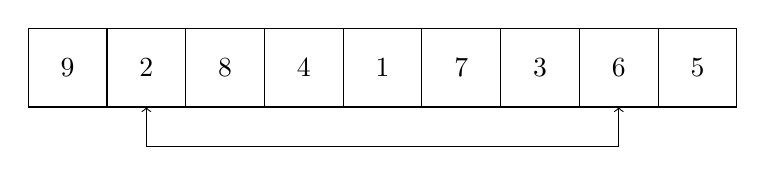
\begin{tikzpicture}
\draw (0, 0) -- (9, 0);
\draw (0, 1) -- (9, 1);

\foreach \i in {0, 1, 2, 3, 4, 5, 6, 7, 8, 9}
	\draw (\i, 0) -- (\i, 1);
	
\draw[<->] (1.5, 0) -- (1.5, -0.5) -- (7.5, -0.5) -- (7.5, 0);

\draw (0.5, 0.5) node{9};
\draw (1.5, 0.5) node{2};
\draw (2.5, 0.5) node{8};
\draw (3.5, 0.5) node{4};
\draw (4.5, 0.5) node{1};
\draw (5.5, 0.5) node{7};
\draw (6.5, 0.5) node{3};
\draw (7.5, 0.5) node{6};
\draw (8.5, 0.5) node{5};
\end{tikzpicture}

Především si povšimněme, že pořadí prvků 2 a~6 se nezmění vůči prvkům ležícím před prvkem 2 a~vůči prvkům ležícím za prvkem 6. Ke změnám inverzí tedy dochází jen mezi nimi:

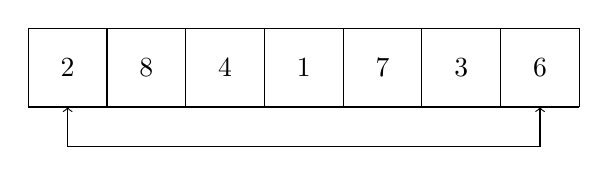
\begin{tikzpicture}
\draw (0, 0) -- (7, 0);
\draw (0, 1) -- (7, 1);

\foreach \i in {0, 1, 2, 3, 4, 5, 6, 7}
	\draw (\i, 0) -- (\i, 1);
	
\draw[<->] (0.5, 0) -- (0.5, -0.5) -- (6.5, -0.5) -- (6.5, 0);

\draw (0.5, 0.5) node{2};
\draw (1.5, 0.5) node{8};
\draw (2.5, 0.5) node{4};
\draw (3.5, 0.5) node{1};
\draw (4.5, 0.5) node{7};
\draw (5.5, 0.5) node{3};
\draw (6.5, 0.5) node{6};
\end{tikzpicture}

Dále si uvědomme, že čísla která jsou menší než číslo 2, jsou také menší než číslo 6. Záměnou prvku 2 za prvek 6 se tedy nezmění inverze s~prvky menšími než 2. Obdobně to platí pro prvky větší než 6. Počet inverzí s prvky ležící mimo aritmetický interval dvou prohazovaných čísel se proto nezmění. Stačí tedy uvažovat jen prvky ležící v~něm:


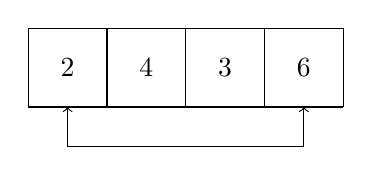
\begin{tikzpicture}
\draw (0, 0) -- (4, 0);
\draw (0, 1) -- (4, 1);

\foreach \i in {0, 1, 2, 3, 4}
	\draw (\i, 0) -- (\i, 1);
	
\draw[<->] (0.5, 0) -- (0.5, -0.5) -- (3.5, -0.5) -- (3.5, 0);

\draw (0.5, 0.5) node{2};
\draw (1.5, 0.5) node{4};
\draw (2.5, 0.5) node{3};
\draw (3.5, 0.5) node{6};
\end{tikzpicture}

Prozkoumejme změnu počtu inverzí s~některým ze zbývajících prvků, například s~prvkem 4. Před prohozením prvků 2 a~6 nejsou s~prvkem 4 žádné inverze, prohozením prvků 2 a~6 vzniknou inverze \((6, 4)\) a~\((4, 2)\). Povšimněme si, že takto vznikne nebo zanikne sudý počet inverzí - buď budeme mít konfiguraci \((2, ..., 4, ..., 6)\) bez inverzí nebo \((6, ..., 4, ..., 2)\) se dvěma inverzemi s~prvkem 4. Je to dáno tím, že prvek 4 leží aritmeticky i~pozičně mezi prvky 2 a 6 - důsledek naší předchozí úvahy o~prvcích mimo. Sudý počet inverzí vznikne nebo zanikne i~vůči ostatním prvkům. Plus vznikne nebo zanikne 1 inverze mezi prvky 2 a 6. Celkově se tedy počet inverzí změní o~lichý počet. 

\begin{fact}
Počet inverzí permutace se prohozením libovolných dvou prvků změní o~lichý počet. 
\end{fact}

To nám umožňuje rozdělit permutace na sudé a~liché:

\begin{fact}
Sudá permutace má sudý počet inverzí, lichá permutace má lichý počet inverzí. Prohozením dvou libovolných prvků se ze sudé permutace stane lichá a~naopak.
\end{fact}

Mějme \(n\) vektorů \(\vect{a}\), \(\vect{b}\), \(\vect{c}\), ... se složkami \(a_i\), \(b_j\), \(c_k\) atd. Pro každou permutaci utvoříme součin \(a_i \cdot b_j \cdot c_k \cdot ...\), kde indexy \(i, j, k, ...\) odpovídají prvkům permutace. Pokud se jedná o~lichou permutaci, tak součin násobíme \(-1\). Tedy pro permutaci \([1, 3, 2]\) budeme mít součin \(-a_1 \cdot b_3 \cdot c_2\). Udělejme součet takovýchto součinů pro všechny permutace. Pro \(n=3\) tedy získáme \(s = a_1 b_2 c_3 + a_2 b_3 c_1 + a_3 b_1 c_2 - a_1 b_3 c_2  - a_3 b_2 c_1 - a_2 b_1 c_3\).

Pokud bychom vektory uspořádali do matice, pak by uvedený součen součinů byl roven jejímu determinantu, tedy:

\begin{equation}
s = 
\begin{vmatrix}
a_1 & a_2 & a_3 \\
b_1 & b_2 & b_3 \\
c_1 & c_2 & c_3 \\
\end{vmatrix}
\end{equation}

Povšimněme si, co se stane, pokud by 2 vektory byli shodné, například pokud \(\vect{a} = \vect{b}\). Počítali-bychom determinant: 

\begin{equation}
s = 
\begin{vmatrix}
b_1 & b_2 & b_3 \\
b_1 & b_2 & b_3 \\
c_1 & c_2 & c_3 \\
\end{vmatrix}
\end{equation}

Získáme tak součet \(s = b_1 b_2 c_3 + b_2 b_3 c_1 + b_3 b_1 c_2 - b_1 b_3 c_2  - b_3 b_2 c_1 - b_2 b_1 c_3 = 0\). Vidíme, že součet je nulový, protože každý jeho člen se v~součtu objevuje jednou s~kladným znaménkem a~jendou se záporným znaménkem. To je důsledkem toho, že sme zavedli součet jako součet všech permutací. Například člen \(+b_1 b_2 c_3\) odpovídá sudé permutaci \(123\) a~člen \(-b_2 b_1 c_3\) liché permutaci \(213\). Protože tyto dvojice členů vzniknou tak, že prohodíme 2 prvky permutace, tak vždy jeden člen bude odpovídat sudé permutaci a~druhý liché permutaci. Proto budou mít vždy opačné zneménko. Obecně proto platí, že takto utvořený součet se dvěma stejnými vektory, tedy determinant matice se dvěma stejnými řádky, je nulový.

Zaveďme Levi-Civitův symbol \(\varepsilon_{ijk...}\):

\begin{fact}
Symbol \(\varepsilon_{ijk...}\) má v~\(n\)-rozměrném prostoru hodnotu \(n\) indexů \(i, j, k, ...\), které mohou nabývat hodnot \(1\) až \(n\). Tvoří-li indexy sudou permutací čísel \(1, 2, ..., n\), pak \(\varepsilon_{ijk...} = +1\). Tvoří-li indexy lichou permutaci, pak \(\varepsilon_{ijk...} = -1\). Netvoří-li indexy permutaci čísel \(1, 2, ..., n\), pak \(\varepsilon_{ijk...} = 0\). Tento případ nastává pokud 2 nebo více indexů je shodných.
\end{fact}

Ve třírozměrném prostoru tedy máme:

\begin{equation}
\begin{split}
\varepsilon_{123} = \varepsilon_{231} = \varepsilon_{312} = +1 \\
\varepsilon_{132} = \varepsilon_{213} = \varepsilon_{321} = -1 \\
\varepsilon_{iij} = \varepsilon_{iji} = \varepsilon_{jii} = 0
\end{split}
\end{equation}

Levi-Civitův symbol nám umožňuje zapsat součet součinů permutací složek \(n\) vektorů. Pro \(n = 3\) máme:

\begin{equation}
s = \sum_{i=1}^3 \sum_{j=1}^3 \sum_{k=1}^3 a_i b_j c_k \varepsilon_{ijk}
\end{equation}

Tuto rovnici můžeme rozepsat na 2:

\begin{equation}
\begin{split}
v_i = \sum_{j=1}^3 \sum_{k=1}^3 b_j c_k \varepsilon_{ijk} \\
s = \sum_{i=1}^3 a_i \cdot v_i
\end{split}
\end{equation}

Získáme tak vektor \(\vect{v}\).
Povšimněme si, že pokud zvolíme \(\vect{a} = \vect{b}\), pak \(s = \sum_{i=1}^3 \sum_{j=1}^3 \sum_{k=1}^3 b_i b_j c_k \varepsilon_{ijk} = 0\). To ale znamená, že \(s = \sum_{i=1}^3 b_i \cdot v_i = 0\), tedy vektor \(\vect{v}\) je kolmý na vektor \(\vect{b}\).

Obdobnou úvahou zjistíme, že vektor \(\vect{v}\) je kolmý na vektor \(\vect{c}\). Ve třírozměrném prostoru proto můžeme zavést tzv. vektorový součin, který utvoří vektor kolmý na 2 vektory:

\begin{equation}
\label{eq:vektorovy_soucin}
\begin{split}
\vect{v} = \vect{b} \times \vect{c} \\
v_i = \sum_{j=1}^3 \sum_{k=1}^3 b_j c_k \varepsilon_{ijk}
\end{split}
\end{equation}

Tuto rovnici můžeme rozepsat na jednotlivé složky uvědomíme-li si, že pouze 6 trojic indexů \(i, j, k\) odpovídá nenulovým \(\varepsilon_{ijk}\):

\begin{equation}
\begin{split}
\vect{v} = \vect{b} \times \vect{c} = \\
(b_2 c_3 - b_3 c_2, b_3 c_1 - b_1 c_3, b_1 c_2 - b_2 c_1) = \\
(b_y c_z - b_z c_y, b_z c_x - b_x c_z, b_x c_y - b_y c_x)
\end{split} 
\end{equation}
